\subsection{Exploring the Wonders of Extended Double Zepp Antennas!}

\begin{tcolorbox}[colback=gray!10, colframe=black, title=E9C12] Which of the following describes an extended double Zepp antenna?
\begin{enumerate}[label=\Alph*.]
    \item An end-fed full-wave dipole antenna
    \item A center-fed 1.5-wavelength dipole antenna
    \item \textbf{A center-fed 1.25-wavelength dipole antenna}
    \item An end-fed 2-wavelength dipole antenna
\end{enumerate} \end{tcolorbox}

\subsubsection{Concepts Related to Extended Double Zepp Antennas}

To understand the nature of an extended double Zepp antenna, we first need to familiarize ourselves with a few key concepts in antenna theory. Antennas are designed to transmit or receive radio waves, and their characteristics often depend on their length and feeding mechanism.

The term center-fed indicates that the antenna is fed with its feed line at its midpoint, allowing for balanced loading on both sides of the antenna. The length of a dipole antenna plays a critical role in determining its performance, including its radiation pattern and impedance.

An extended double Zepp antenna specifically refers to a dipole configuration where the effective electrical length exceeds that of a standard half-wave dipole. In this case, an extended double Zepp antenna is typically around 1.25 wavelengths long. This particular length can enhance the gain and directivity of the antenna compared to a standard dipole antenna.

\subsubsection{Calculation of Wavelength}

To grasp the notion of the antenna length mentioned, we can calculate its physical length in accordance with the wavelength of the radio frequency of interest using the following formula:

\[
L = \frac{468}{f(MHz)}
\]

Where:
- \(L\) is the length of the dipole antenna in feet,
- \(f\) is the frequency in megahertz (MHz).

For example, if we are working with a frequency of 2 MHz, we would first calculate the standard dipole length:

\[
L = \frac{468}{2} = 234 \text{ feet}
\]

For an extended double Zepp antenna, specifically 1.25 times the standard half-wave length, we find:

\[
L_{EDZ} = 1.25 \times 234 = 292.5 \text{ feet}
\]

This indicates that an extended double Zepp antenna tuned for 2 MHz would ideally have a total length of approximately 292.5 feet. 

\subsubsection{Diagram of an Extended Double Zepp Antenna}

Here is a simple representation of the extended double Zepp antenna using the TikZ package:

\begin{center}
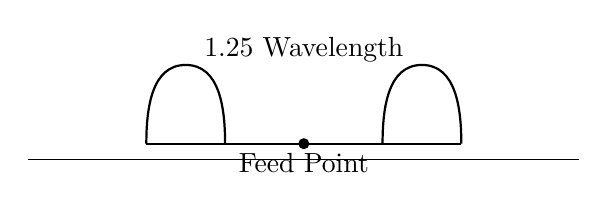
\begin{tikzpicture}
    % Draw the antenna
    \draw[thick] (0,0) -- (4,0); % Main part of Dipole
    \draw[thick] (0,0) to[out=90,in=180] (0.5,1) to[out=0,in=90] (1,0); % Left side curve
    \draw[thick] (4,0) to[out=90,in=0] (3.5,1) to[out=180,in=90] (3,0); % Right side curve
    
    % Label the feeding point
    \fill (2,0) circle (2pt);
    \node[below] at (2,0) {Feed Point};

    % Draw the ground
    \draw[-] (-1.5,-0.2) -- (5.5,-0.2);
    
    % Label the antenna length 
    \node at (2,1.2) {1.25 Wavelength};
\end{tikzpicture}
\end{center}

In summary, an extended double Zepp antenna is characterized distinctly by its length and feeding mechanism, which provides a unique balance of performance in radio communication applications.
